\documentclass[a4paper,10pt]{article}
%\documentclass[a4paper,10pt]{scrartcl}

\usepackage[utf8]{inputenc}
\usepackage{graphicx}
\usepackage[demo]{graphicx}
\usepackage{caption}
\usepackage{subcaption}


\title{Introduction to machine learning}
\author{Herkko Virolainen, 013463430}
\date{}

\pdfinfo{%
  /Title    ()
  /Author   ()
  /Creator  ()
  /Producer ()
  /Subject  ()
  /Keywords ()
}

\begin{document}
\section {perceptron, mnist set}

Ensimmäisenä tehtävä oli luoda perceptron algoritmi, jota sitten käytetään käsinkirjoitettujen numeroiden luokitteluun. Tässä tapauksessa tarkoituksena
oli luokitella ainoastaan 1 ja 0. Tein toteutuksen Matlabilla. Tein numeroiden lataamiseen oman scriptin, joka valitsee numeroista vain 1 ja 0, 
ja jakaa pikselidatan sekä oikeat luokat omiin muuttujiinsa. Tämän lisäksi on itse perceptron funktio omassa tiedostossaan, joka hoitaa luokittelijan
opettamisen. Sitten on vielä classifier funktio, jolla voi luokitella käyttäen aiemmin luotua luokittelijaa. 

Algoritmi on kaikessa yksinkertaisuudessaan seuraava. Valitaan luokittelijaksi alustusvaiheessa ensimmäinen luokiteltava alkio. Tämän jälkeen käydään yksi
kerrallaan alkioita läpi ja verrataan niitä luokittelijaan. Jos luokittelija luokittelee alkion oikein, ei tehdä mitään. Jos luokittelija luokittelee
alkion väärin, lisätään kyseinen alkio luokittelijaan. Luokittelijan vektori tällöin kääntyy kohti sellaista vektroia joka olisi luokitellut kyseisen alkion oikein.
Tätä jatketaan niin kauan, kunnes käydään kaikki luokiteltavat alkiot läpi ilman että luokittelijaa tarvitsee muuttaa. Jos aineisto on lineaarisesti eroteltavissa, niin
sopiva luokittelija löytyy aina. 


Testatessa ensimmäisenä tein 2-uloitteisia testiaineistoja, jotta tiedän toimiiko luokittelija. Kaikissa seteissä pisteitä oli senverran vähän että jos 
luokat olivat eroteltavissa, niin algoritmi konvergoi parissa iteaatiossa. Seuraavalla sivulla on muutamia kuvia, joista näkee minkälaisia 
ryhmiä luokittelija sai luotua. Kohtasin pieniä ongelmia siinä miten olisin saanut MatLabissa esitettyä pisteet omina luokkinaan, mutta 
tässä tapauksessa onneksi pisteitä on niin vähän, että on melko selvää mitkä pisteet kuuluvat mihinkin luokkaan. Tarkastin kuitenkin käsin, että 
saadut tulokset olivat järkeviä.
\begin{figure}[ht]

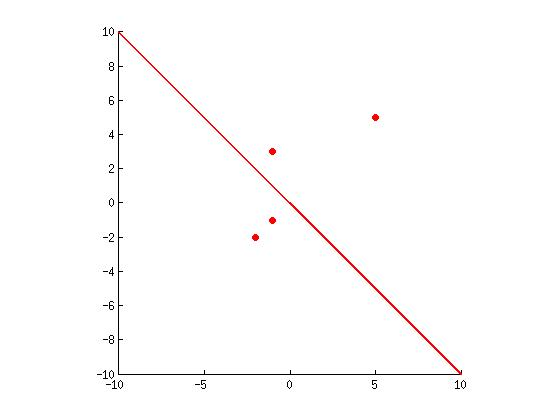
\includegraphics[width=70mm]{sanityCheck1.jpg}
\caption{Luokittelijan testi 1}


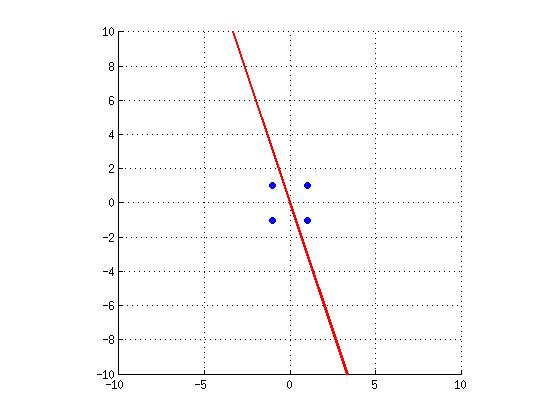
\includegraphics[width=70mm]{sanityCheck2.jpg}
\caption{Luokittelijan testi 2}

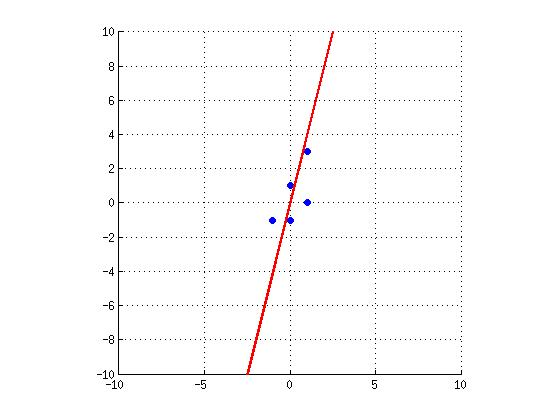
\includegraphics[width=70mm]{sanityCheck3.jpg}
\caption{Luokittelijan testi 3, Kaikista toimivista luokista tässä oli pienin marginaali.}

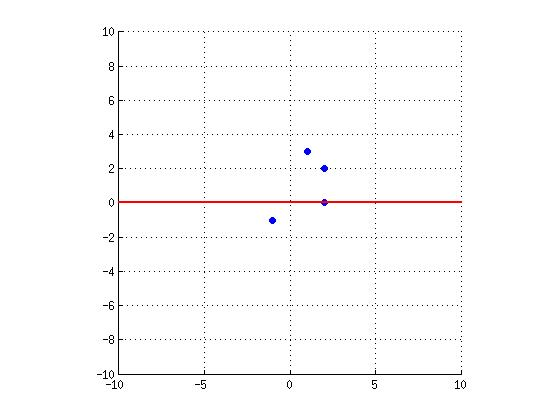
\includegraphics[width=70mm]{sanityCheck4.jpg}
\caption{Pisteet eivät olleet luokiteltavissa, algoritmi ei konvergoinut}


\end{figure}
\clearpage 


Seuraavaksi latasin apufunktiolla 5000 datapistettä mnist aineistosta ja otin sieltä vain 1 ja 0.
Opetusaineistoon ja testiaineistoon tuli kumpaankin noin 500 alkiota. Perceptron algoritmi konvergoi toisella iteraatiolla. Tämän jälkeen kun luokittelijan
antoi syötteenä testiaineistolle, oli virheprosentti 0\%.
Tulos ei sinällään ollut kovin yllättävä, koska aineiston dimensio oli todella suuri, sekä 1 ja 0 ovat melko kaukana toisistaan jos asiaa miettii 
pikselitasolla. Visualisaatio paketti oli joko jotenki rikki tai en osannut vain käyttää sitä, mutta en onnistunut luomaan kuvaa esimerkin mukaisesti yksittäisistä
numeroista, enkä luokittelijasta,niinkuin tehtävänannossa pyydettiin. Uskoisin kuitenkin että luokittelija ei juurikaan näytä kummaltakaan numerolta, vain jonkinlaiselta
sekoitukselta kummastakin. 
\newline

Koodin testaus onnistuu esimerkiksi seuraavanlaisilla komennoilla.
\begin{itemize}
\item - [testNumbers, trainNumbers, testclasses, trainclasses] =  helpLoadingNumbers()
\item classifier = perceptron(trainNumbers,testClasses)
\item classify(classifier, testNumbers, testClasses)

\end{itemize}




\section{Bayes classifier, news set}

Toisessa tehtävässä oli tarkoitus luoda yksinkertainen Bayes luokittelija, joka luokittelee dokumentteja kuulumaan erilaisiin uutisryhmiin perustuen 
dokumentin sisältöön. 
Ensimmäiseksi luotiin harjoitus setti, jonka avulla bayes luokittelijaa lähdetään opettamaan. Settiin valittiin jokaisesta uutisryhmästä 90\% dokumenteista. 
Tämän jälkeen jokaiselle sanalle laskettiin todennäköisyys kuulua tiettyyn uutisryhmään sen perusteella kuinka monessa uutisryhmän dokumentissa kyseinen sana esiintyi. Kun kaikki 
dokumentit oli käyty läpi, oli luokittelija valmis. Luokittelijaa voi käyttää siten, että katsoo dokumentin sanojen todennäköisyydet kuulua uutisryhmiin ja se 
uutisryhmä joka saa suurimman todennäköisyyden on valittu luokka. 

Yllätykseksi Luokittalija toimi todella huonosti. En osaa sanoa johtuiko se jostain implementointivirheestä tai muuta vastaavaa, mutta luokittelija onnistui luokittelemaan
oikein kohtalaisella prosentilla vain muutamat luokat: 11,12, 16,17, 18 ja 19. Lopuilla oikein luokiteltujen dokumenttien määrä oli lähellä 0\%.

Jos implementaatiossani ei ollut mitään vikaa ja tämä oli odotettava tulos, niin olen vähintäänkin hämmentynyt. Oletin että luokittelija olisi ollut parempi tällaisen aineiston kanssa.
Algoritmia voi testata seuraavilla komennoilla
\begin{itemize}
\item  [Xs y voc groups] = loadnews();
\item . [classifier, trainingSet, testSet] = bayes(voc, Xs, y);
\item result = classify(voc, Xs, testSet, classifier)
\end{itemize}

\section{Hierarial clustering, movie dataset}
Kolmantena tehtävänä oli tehdä clusterointi algoritmi, joka luokittelee elokuvia samoihin luokkiin katsojien antamien suositusten perusteella.
Tein ohjelman kotona matlabilla, jossa minulla ei ollut saatavilla statistical toolboxia, joten dendrogrammien tekeminen ei onnistunut, joten jouduin
tulkitsemaan kaikki luomani esimerkit ruutupaperille. 

\newline

Ensimmäisenä kokeilin algoritmia 5x5 matriisiin, johon olin laskenut käsin sopivia pisteiden etäisyyksiä, niin että niiden oikeellisuus olisi helppo
tarkistaa suoraa ruutupaperilta. Tein esimerkin myös siten, että klustereista tulisi tarpeeksi erilaisia riippuen siitä pyydetäänkö algoritmia
toimimaan single link vai multilink mallilla. Klusterit näyttivät toimivan juuri niinkuin pitääkin, joten siirryin elokuvien pariin. Etsin elokuvista
muutaman selkeästi lasten elokuvan kuten Toy Storyn, 101 dalmatialaista ja niin edelleen. Toisena selkeänä ryhmänä valitsin mukaan Star Trek elokuvia, joiden
kuvittelin olevan Jaccrd Coefficient mielessä melko lähellä toisiaan. Samaa genreä mukaillen otin mukaan myös Aliens elokuvat.
Muuten valitsin mukaan satunnaisia elokuvia, kuitenkin niin että ne olisivat hieman erilaisia kuin jo valitut elokuvat.

Tälle setille kummallakin tavalla tuotettu tulos oli melko samannäköinen. Vain pienehköjä eroja miten klusterit olivat muodostuneet. Tämä oli toisaalta melko odotettu tulos, koska erot 
eri elokuvien välillä ovat melko samansuuruisia, joten mitään kovin isoja eroja ei voi odottaa muuttamalla klusterointitaktiikkaa. 


\begin{figure}[klusterit]

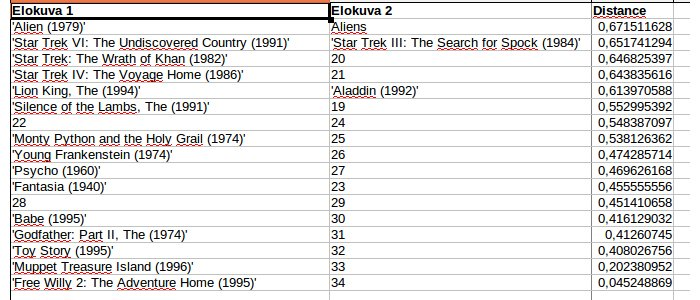
\includegraphics[width=150mm]{movies.jpg}
\caption{Complete-link klusteroidut elokuvat}

\end{figure}
\begin{figure}[klusterit]

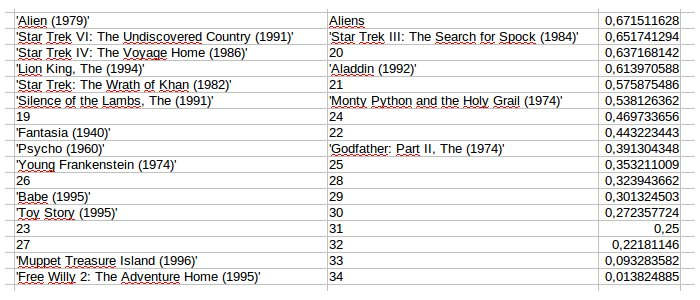
\includegraphics[width=150mm]{moviessl.jpg}
\caption{Single-link klusteroidut elokuvat}

\end{figure}

\end{document}
